\chapter{Binomial Tree Methods}

[Deleted parts that are moved over]

\section{Visualisation}

We are now ready to visualise our binomial tree model. Figure \ref{fig:tree_plot1} plots the option values across different asset prices and different times. We can see that at $t=1$, we are at expiry and hence the value is just the intrinsic value. However, the further we are from expiry, the more the option is worth. This is because the option has time value: the more time we have left to expiry, the more optionality we have and the more opportunity the asset has to be in the money. This additional optionality costs, and hence we can see that the put option loses value over time even if the asset price stays the same.

This phenomenon can be examined more closely in \ref{fig:tree_plot2}. We examine the structures for in the money, at the money and out of the money put options. We supply the European price for reference, and we can see that the European price indeed bounds the American price from below as we'd expect. We can see that the option loses value as we approach maturity. An interesting figure to examine is the in the money figure: we can see that the value flattens at $0.1$, the intrinsic value of the option, at some time $t^\star \in (0, 1)$. This is the point of time beyond which it is always beneficial to perform early exercise, and hence the value of the option is just the intrinsic value. At times $0<t < t^*$ the option is worth more as we have the option to wait, giving the option time value.

\begin{figure}[h]
    \centering
    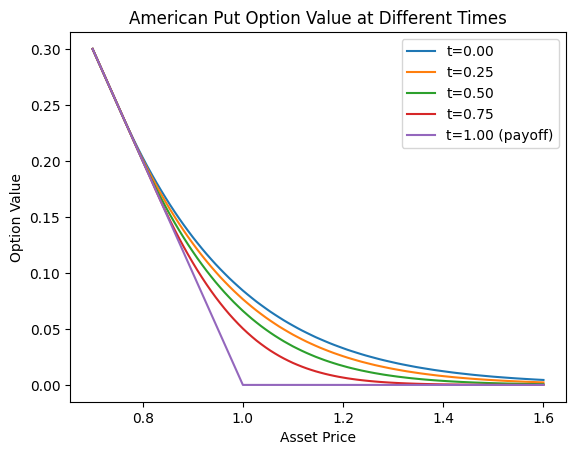
\includegraphics[width=0.5\textwidth]{../plots/binomial_tree/tree_plot1.png}
    \caption{Option value on different asset prices across time}
    \label{fig:tree_plot1}
\end{figure}

\begin{figure}[h]
    \centering
    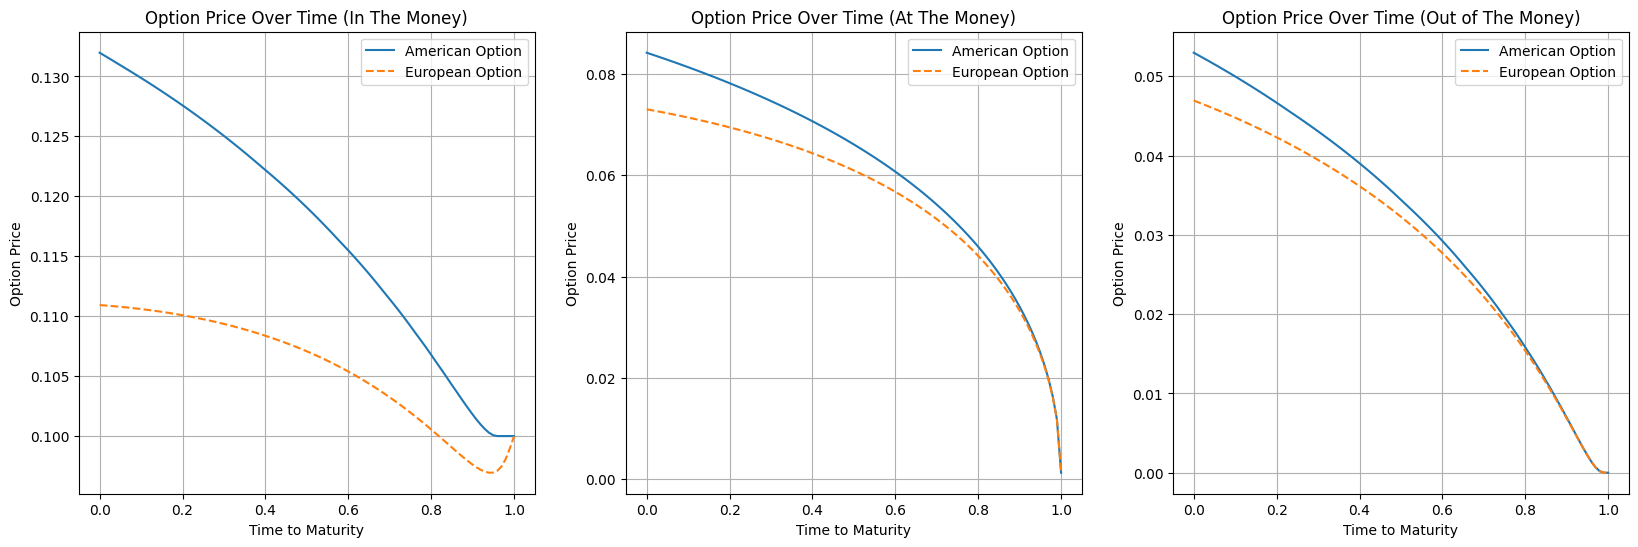
\includegraphics[width=\textwidth]{../plots/binomial_tree/tree_plot2.png}
    \caption{Decay in time value}
    \label{fig:tree_plot2}
\end{figure}
